\input{configuration}

\title{Lecture 5 --- More SQL }

\author{Jeff Zarnett \\ \small \texttt{jzarnett@uwaterloo.ca}}
\institute{Department of Electrical and Computer Engineering \\
  University of Waterloo}
\date{\today}


\begin{document}

\begin{frame}
  \titlepage

 \end{frame}



\begin{frame}
\frametitle{String Operations}

String operations are complicated in any language and SQL is no exception. 

\begin{center}
	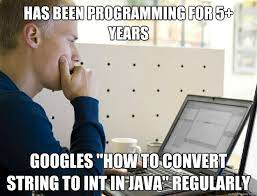
\includegraphics[width=0.6\textwidth]{images/strings.jpg}
\end{center}

 \end{frame}



\begin{frame}
\frametitle{String Operations}


We used some string matching already so we have a good idea how it works: 

By default a string is enclosed in single-quote characters such as \texttt{'AAAA 111'}. 

Double quotes can also be used, especially if you need to enclose a single-quote literal in your string such as: \texttt{"Burk's Falls"}.

\end{frame}



\begin{frame}
\frametitle{String Operations}

The SQL standard says that string comparison with \texttt{=} is case sensitive.


MySQL (and some others) do not respect this and perform case-insensitive comparison. 

\begin{center}
	
\includegraphics[width=0.4\textwidth]{images/table-flip.jpg}
\end{center}

\end{frame}



\begin{frame}
\frametitle{String Operations}


Standards are optional, I guess? 

MySQL has gotten better and made this a configurable parameter, but it's still something to be wary of.


\end{frame}



\begin{frame}
\frametitle{Sring Operations}

Some functions familiar from C-like languages exist:\\
\quad  \texttt{UPPER()}, \texttt{LOWER()}, \texttt{TRIM()}, et cetera. 

Pattern matching can be done using \texttt{LIKE} which takes two special characters as wildcards: \texttt{\%}, and \texttt{\_}.  

If you need those characters explicitly, they are escaped using the \textbackslash~ as one might expect. 

The backslash itself can also be escaped using the backslash.

\end{frame}


\begin{frame}
\frametitle{String Operations}

Some examples might clarify how it works: the clause \texttt{LIKE 'Marc\%'} would match the strings ``Marc'', ``Marco'', ``Marcelline'', and so on. 

The clause \texttt{LIKE 'Marc\_'} would match only ``Marco'' from that previous set (exactly one character is required). 


\end{frame}



\begin{frame}
\frametitle{Null Bottles of Beer on the Wall...}

A null attribute indicates a lack of a value and it causes a certain chaos with some of our operations.

Arithmetic expressions involving null (e.g., addition, subtraction, etc) always results in null if any one of the operands is null. 

Comparisons involving null are also a hassle; saying whether 1 is ``less than'' null is not sensible so the value will be ``unknown''.

\end{frame}



\begin{frame}
\frametitle{Unknown is the Loneliest Non-Number}

Use of ``unknown'' values in boolean operators is also complicated:

\begin{itemize}
	\item  AND: Comparing true AND unknown results in unknown; false AND unknown results in false; unknown AND unknown results in unknown. \\[3em]
	\item OR: Comparing true OR unknown results in true; false OR unknown results in unknown; unknown OR unknown results in unknown. \\[3em]
	\item NOT unknown also results in unknown.
\end{itemize}

\end{frame}



\begin{frame}
\frametitle{Testing (Not-)Nullity}

If a where clause for a particular tuple evaluates to false, it is not added to the tuples to be returned or changed. 

It is possible, though, to test whether something is null, or is not null. 

\begin{center}
	
\includegraphics[width=0.5\textwidth]{images/nospoon.jpg}
\end{center}



\end{frame}



\begin{frame}
\frametitle{Testing (Not-)Nullity}

As you might expect, those are \texttt{IS NULL} and \texttt{IS NOT NULL}. 


Example: \texttt{SELECT * from VEHICLE WHERE year IS NULL;}.

It is correct to use the \texttt{IS NULL} or \texttt{IS NOT NULL} constructions rather than something like \texttt{= null} or \texttt{<> null}.

\end{frame}



\begin{frame}
\frametitle{Medium Double-Double}

If multiple tuples are returned by a query, we get them in no specified order. 

You may see consistent behaviour across repeated queries, but no promises are made about the order in which they are delivered. 


\begin{center}
	
\includegraphics[width=0.4\textwidth]{images/order.jpg}
\end{center}

We can change that, if we want, through the use of an \texttt{ORDER BY} clause. 

\end{frame}



\begin{frame}
\frametitle{Medium Double-Double}


We specify the attribute to sort by, and we can choose ascending (\texttt{ASC}) or descending (\texttt{DESC}). 

An example: \texttt{SELECT * FROM VEHICLE ORDER BY make ASC}.

\end{frame}



\begin{frame}
\frametitle{Multiple Orders}

We may specify multiple attributes in the \texttt{ORDER BY} clause, such as \texttt{ORDER BY make DESC, model DESC}. 

This sorts by the ``make'' attribute (descending), and if the values of two tuples are equal in that attribute, then by ``model'' (descending). 


\end{frame}



\begin{frame}
\frametitle{Multiple Orders}

If no two tuples have the same 1st sort attribute, the 2nd sort does nothing.

You can choose divergent directions: mixing ascending and descending.

The field used to order the tuples does not have to be returned in the result set.


\end{frame}



\begin{frame}
\frametitle{Aggregation}

\begin{center}
	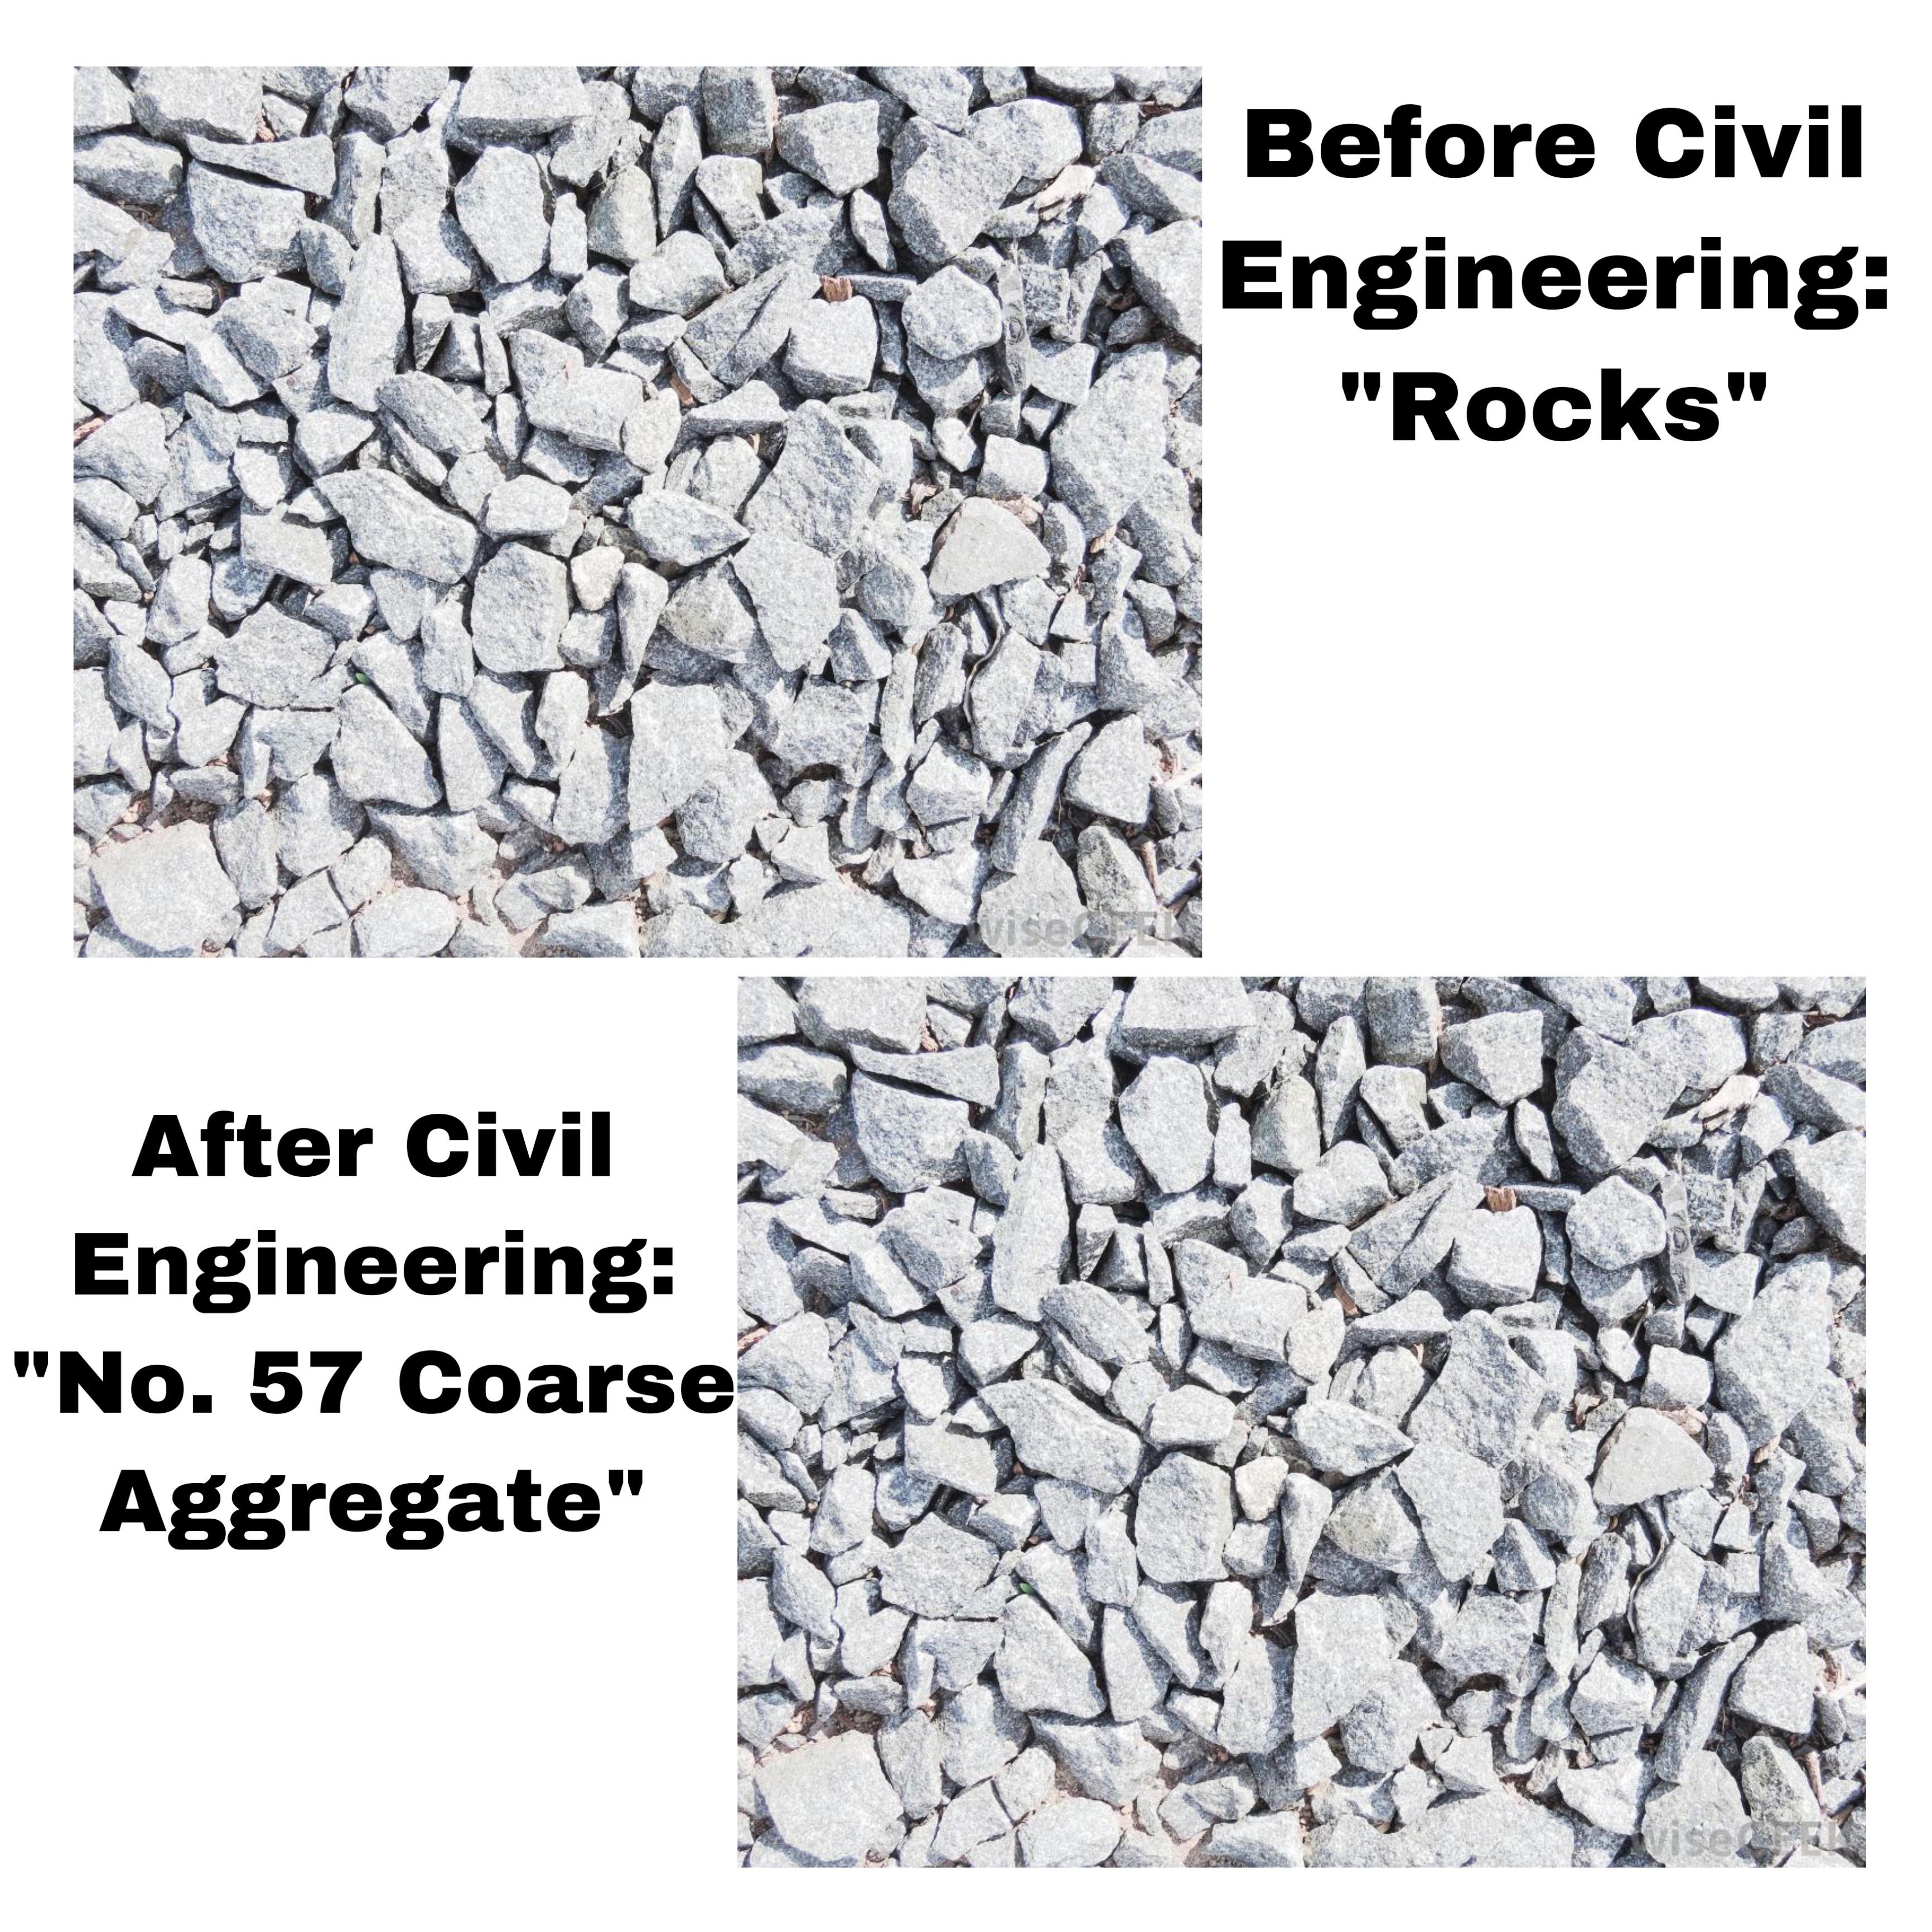
\includegraphics[width=0.7\textwidth]{images/civileng.jpg}
\end{center}


\end{frame}



\begin{frame}
\frametitle{Aggregation}

Aggregate functions perform a reduction on the data. 

If you are given an array of integers and asked to sum it up, that's a reduction. 

\begin{center}
	
\includegraphics[width=0.3\textwidth]{images/reduction.jpg}
\end{center}

\end{frame}



\begin{frame}
\frametitle{Aggregation}

The aggregate functions in SQL mostly are:
\begin{enumerate}
	\item \texttt{AVG}: Average 
	\item \texttt{MAX}: Maximum
	\item \texttt{MIN}: Minimum
	\item \texttt{SUM}: Sum (total)
	\item \texttt{COUNT}: Count (obviously)
\end{enumerate}


\end{frame}



\begin{frame}
\frametitle{Aggregation}

These work more or less like you would expect: 

You can \texttt{SELECT SUM( salary ) FROM employee;} to get the total salary of all employees, 

Or \texttt{SELECT AVG( salary ) FROM employee;} to get the average salary of all employees.

Maximum and minimum are also pretty self-explanatory. 

Sum and average work only on numbers, but non-numeric types can be used for maximum and minimum. 

\end{frame}


\begin{frame}
\frametitle{Select Count...}

\texttt{SELECT COUNT( salary ) FROM employee;} tells you the number of entries in the table where there is a salary. 

More commonly you would see \texttt{SELECT COUNT(*)} to count the number of entries in the relation.

You could also put the primary key in the parenthesis instead of the asterisk if the asterisk gives you worries about performance nightmares.


\end{frame}



\begin{frame}
\frametitle{Select Count Distinct...}

One can also put \texttt{DISTINCT} in the count expression. 

If you wished to count the number of distinct model names, you could write \texttt{SELECT COUNT( DISTINCT make ) FROM vehicle;} which would remove duplicates.

SQL does not permit combination of \texttt{DISTINCT} and \texttt{COUNT(*)}.\\ \quad Although it seems like this is accepted by MySQL.

\end{frame}



\begin{frame}
\frametitle{Group and Sum}

It is nice to be able to sum up or average over all tuples matching some clause, but we can get grouping if we want as well. 

It might be interesting to know there are 150 different models of car. 

If we are curious we can add a where clause to find out how many are made by Audi, and then another one where we find out how many are made by BMW... 

But that is inefficient. The solution is grouping.


\end{frame}



\begin{frame}
\frametitle{Group and Sum}

\texttt{SELECT make, COUNT(model) FROM vehicle GROUP BY make;} might produce a result like the table shown below:

\begin{center}
\begin{tabular}{|l|l|}\hline
	\textbf{make} & \textbf{count(model)} \\ \hline
	Honda & 1  \\ \hline
	Ford & 1  \\ \hline
	Volkswagen & 2  \\ \hline
	Totoya & 1  \\ \hline
	Chevrolet & 1  \\ \hline
	Genesis & 1  \\ \hline
\end{tabular}
\end{center}

\end{frame}



\begin{frame}
\frametitle{Restrictions on Aggregation Queries}

The select statement selects over some attributes of the relation and they must be either (1) in the group by clause or (2) aggregated in some way. 

The statement \texttt{SELECT make, COUNT(model), year FROM vehicle GROUP BY make;} is invalid.

The attribute ``year'' is not in the group by clause nor is it aggregated. 

This is sensible: there are multiple values for the ``year'' attribute and we would have no way of knowing which is the correct value to output here.

\end{frame}


\begin{frame}
\frametitle{Aggregation and Having}

That's nice, but what if we wanted to return only those rows where a certain property holds, such as count is greater than 1? 

For that there is the \texttt{HAVING} clause which would be applied as follows: 

\texttt{SELECT make, COUNT(model) FROM vehicle GROUP BY make HAVING COUNT(model) > 1;} 

This would return only the one tuple (Volkswagen).

\end{frame}



\begin{frame}
\frametitle{Breaking Down the Query}

\begin{enumerate}
	\item The \texttt{FROM} clause is evaluated to get the relation.
	\item The \texttt{WHERE} clauses is evaluated on the tuples in the relation specified in the \texttt{FROM} clause.
	\item Tuples matching the \texttt{WHERE} clause are placed into groups according to the \texttt{GROUP BY} clause (if this is absent, then it's all one big group).
	\item The \texttt{HAVING} clause, if any, is evaluated and removes groups that don't meet the having condition.
	\item The \texttt{SELECT} operation is performed, producing the tuple for each group.
\end{enumerate}

\end{frame}



\begin{frame}
\frametitle{Aggregation and Null}


In general, aggregate operations on null values tend to ignore any nulls they encounter.

If the SQL query sums salaries and there is a null value it will not affect the sum (i.e. it will be treated like zero). 

The \texttt{COUNT} function does not, however. 

As usual, nulls have the potential to cause chaos.

\end{frame}



\begin{frame}
\frametitle{Subqueries and Set Comparison}

We can have subqueries (nested queries) where the result of one query is used as input to another query in a single statement. 

The keyword we are going to use extensively here is \texttt{IN}.  

\texttt{SELECT * FROM employee WHERE id = 2419 OR id = 2917 OR id = 4058 OR id = 5911;} becomes instead:


\texttt{SELECT * FROM employee WHERE id IN (2419, 2917, 4058, 5911);}.

\end{frame}



\begin{frame}
\frametitle{Subquery}

Instead of an explicit list, the list could be generated by a query. 

Suppose the ministry of transport has discovered that license plates in the range CCCC 001 through CCCC 999 were manufactured incorrectly.


\begin{center}
	
\includegraphics[width=0.3\textwidth]{images/subquery.png}
\end{center}


\end{frame}



\begin{frame}
\frametitle{Subquery}


The ministry can send an e-mail to everyone affected to tell them of the problem and offer a free replacement. 

\texttt{SELECT name, street, city, province, postal\_code FROM owner\_address WHERE id IN (SELECT owner\_address\_id FROM license\_plate WHERE number LIKE 'CCCC\%');}



\end{frame}



\begin{frame}[fragile]
\frametitle{Vehicle Recall}
Or for a vehicle recall...?

In that case we need to have three tables linked and we can do that with subqueries.
{\scriptsize
\begin{verbatim}
SELECT name, street, city, province, postal_code 
FROM owner_address WHERE id IN 
  (SELECT id FROM license_plate WHERE number IN 
    (SELECT license_plate_number FROM vehicle WHERE make = 'Volkswagen' AND model = 'Golf')
  );
\end{verbatim}
}

\end{frame}



\begin{frame}
\frametitle{Subquery or Join?}

\begin{center}
	
\includegraphics[width=0.5\textwidth]{images/forkroad.jpg}
\end{center}


We can usually replace a subquery with a join query, and vice versa.

 In many cases it is a question of taste, but sometimes a subquery is easier to read and understand (especially if it is complex). 


\end{frame}



\begin{frame}
\frametitle{Other Things}

This has by no means been an exhaustive list of all the SQL keywords one could possibly use (e.g., \texttt{UNIQUE}, \texttt{WITH}, et cetera). 

We may introduce more syntax later if it is relevant to some other operation. 

For the moment, however, we have enough syntax covered to continue on to modification as well as design. 


\end{frame}


\begin{frame}
\frametitle{Modification}

Until now all the operations we have looked at the data, combined it, sliced and diced it, and generated some temporary values -- but that's it. 

We haven't actually changed the data in any permanent way. 

There are three basic operations we can do: add, remove, and change.
\end{frame}



\begin{frame}
\frametitle{Modification}

\begin{center}
	
\includegraphics[width=0.4\textwidth]{images/change-hard.jpg}
\end{center}

\end{frame}



\begin{frame}
\frametitle{Modification}

Keep in mind that modification operations are transactions. 

These operations can also be expressed using relational algebra with an assignment. 

\end{frame}



\begin{frame}
\frametitle{Insert}

The insert statement creates a new tuple and adds it to the relation, or creates a set of tuples and then adds that set to the relation.

If we are creating just one, then the simple, manual approach is sufficient. 

In SQL the keywords are \texttt{INSERT INTO} and \texttt{VALUES}. 

To add a new license plate we would write: \texttt{INSERT INTO license\_plate( number, expiry, owner\_address\_id ) VALUES( 'HOLMES01', '2018-12-10', 86753 );} 

\end{frame}



\begin{frame}
\frametitle{Not All Attributes}

It is permissible to leave some attributes out of the insert statement. 

\texttt{INSERT INTO license\_plate( expiry, number ) VALUES( '2018-12-10', 'HOLMES01' );} would create a tuple where the owner address id attribute contains null. 

This must, however, be permitted by the table definition: i.e., the field must allow null attributes or have a defined default.


\end{frame}



\begin{frame}
\frametitle{Multiple Insertion}


We may also insert multiple elements into a relation based on the result of a select statement. 

\texttt{INSERT INTO owner\_address ( SELECT * FROM employee\_address )};

This statement leaves off the attribute specification (not recommended) and has no predicate (where clauses) so it is a rather dangerous statement to write.

In relational algebra, if the relation is $r$ and the new tuples are $t$, then the insert statement is $r \leftarrow (r \cup t)$.


\end{frame}


\begin{frame}
\frametitle{Delete}

The delete operation can only be used to remove a set of tuples from a single relation.

It does not alter attributes in the tuples. 

If the goal is to ``clear fields'' the update statement is appropriate. 

A delete statement cannot be used on multiple relations at once.


\end{frame}



\begin{frame}
\frametitle{DELETE}

The keyword in SQL is \texttt{DELETE}.

\begin{center}
	
\includegraphics[width=0.4\textwidth]{images/delete.jpg}
\end{center}

\url{https://www.youtube.com/watch?v=4ecWDo-HpbE}

\end{frame}



\begin{frame}
\frametitle{DELETE}

The statement \texttt{DELETE FROM license\_plate WHERE number = 'BBCC 394';} will remove from the license plate relation any and all tuples that match the predicate. 

If no predicate is specified, then ALL tuples in the relation are removed (yikes!).

\end{frame}



\begin{frame}
\frametitle{Subquery Deletion}


Like an insertion we may use the result of a subquery as the predicate in a where clause. 

We could delete all license plates where the registered address province is not Ontario with something like: 

\texttt{DELETE FROM license\_plate WHERE owner\_address\_id IN (SELECT id FROM owner address WHERE province <> 'ON');}

\end{frame}



\begin{frame}
\frametitle{Delete The Poor People?}

Consider example about deletion where the salary is less than the average. 

This highlights that the deletion operation first figures out the average, then decides what tuples to delete, before carrying out the operation. 

If this were not the case, after each deletion the average might change and we might delete all tuples (or the result would otherwise be strange). 


\end{frame}



\begin{frame}
\frametitle{Deletion}


In relational algebra then the relation $r$ is modified by a deletion with predicate $p$ as follows: $r \leftarrow (r - \sigma_{p}( r ) )$.

Deletion should be used very carefully. When data is removed from the database, it's gone and not coming back.


\end{frame}



\begin{frame}
\frametitle{Update}

The update statement changes one or more attributes of the tuple without changing all the values in the tuple. 

The update statement, like the delete operation, operates on a set of tuples: one may specify the predicate with the \texttt{WHERE} clause just as before. 

In SQL the keywords we need are \texttt{UPDATE} and \texttt{SET}.  

To update someone's address: \texttt{UPDATE OWNER\_ADDRESS SET postal\_code = 'B1B 2B2` WHERE id = '24601';}. 


\end{frame}



\begin{frame}
\frametitle{Update}


It is necessary to specify at least one attribute to change, although it is possible that no tuples are changed because none match the where-predicate. 

Similarly, an update may fail if we try to violate one of the rules. 

If the new text is too long for the attribute...

There are also some rules about updating an identifier for this relation (but we'll come back to this subject).

\end{frame}



\begin{frame}
\frametitle{The Rich Get Richer}

\texttt{UPDATE employee SET salary = salary * 1.50 WHERE id = 1;}. 

This takes the current value of salary for the employee with id ``1'' and increases it by 50\%.

\begin{center}
	
\includegraphics[width=0.5\textwidth]{images/medal.jpg}
\end{center}

(The CEO is ever so generous to the CEO, no?)

\end{frame}



\begin{frame}
\frametitle{The Rich Get Richer}

In this case the attribute salary is both read and written. 

The assignment takes place after the right side expression has been evaluated.

Rather like in C: \texttt{x = x + 5;}

\end{frame}



\begin{frame}
\frametitle{Employees Get Paid}

Similarly, if the statement is \texttt{UPDATE employee SET salary = salary * 1.05 WHERE salary > 100000;}?

The behaviour is like deletion in that the set of salaries to update is determined before any modifications begin. 

The whole statement, no matter how many tuples it affects, is viewed as a transaction. 

We could model this in relational calculus as simultaneous deletion of the old tuple and insertion of the new one. 


\end{frame}







\end{document}

